\documentclass[10pt]{article}
\usepackage[polish]{babel}
\usepackage[utf8]{inputenc}
\usepackage[T1]{fontenc}
\usepackage{amsmath}
\usepackage{amsfonts}
\usepackage{amssymb}
\usepackage[version=4]{mhchem}
\usepackage{stmaryrd}
\usepackage{graphicx}
\usepackage[export]{adjustbox}
\graphicspath{ {./images/} }

\title{Kod ucznia }

\author{}
\date{}


\begin{document}
\maketitle
\(\qquad\)\\
\(\qquad\)

\section*{MATEMATYKA}
28 LUTEGO 2017

\section*{Instrukcja dla zdającego}
Czas pracy:\\
170 minut

\begin{enumerate}
  \item Sprawdź, czy arkusz zawiera 14 stron (zadania 1-34). Ewentualny brak zgłoś przewodniczącemu zespołu nadzorującego egzamin.
  \item Rozwiązania zadań i odpowiedzi zamieść w miejscu na to przeznaczonym.
  \item Odpowiedzi do zadań zamkniętych (1-25) przenieś na kartę odpowiedzi, zaznaczając je w części karty przeznaczonej dla zdającego. Zamaluj pola do tego przeznaczone. Błędne zaznaczenie otocz kółkiem i zaznacz właściwe.
  \item Pamiętaj, że pominięcie argumentacji lub istotnych obliczeń w rozwiązaniu zadania otwartego (26-34) może spowodować, że za to rozwiązanie nie otrzymasz pełnej liczby punktów.
  \item Pisz czytelnie i używaj tylko długopisu lub pióra z czarnym tuszem lub atramentem.
  \item Nie używaj korektora, a błędne zapisy wyraźnie przekreśl.
  \item Pamiętaj, że zapisy w brudnopisie nie będą oceniane.
  \item Możesz korzystać z zestawu wzorów matematycznych, cyrkla i linijki oraz kalkulatora prostego.
  \item Na tej stronie oraz na karcie odpowiedzi wpisz swój kod (nazwisko i imię - zgodnie z ustaleniami szkolnymi).
  \item Nie wpisuj żadnych znaków w części przeznaczonej dla egzaminatora.
\end{enumerate}

Życzymy powodzenia!

Liczba punktów\\
do uzyskania: \(\mathbf{5 0}\)

\section*{LUBELSKA PRÓBA PRZED MATURĄ 2017 - poziom podstawowy}
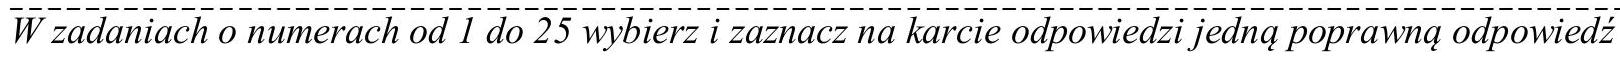
\includegraphics[max width=\textwidth, center]{2024_11_21_d45b0573b36a3462565cg-02(3)}\\
Zadanie 1. (1p)\\
Rozwiązaniem nierówności \(-5 \leq x-2<1\) jest zbiór\\
A\\
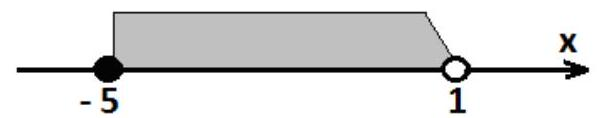
\includegraphics[max width=\textwidth, center]{2024_11_21_d45b0573b36a3462565cg-02(4)}\\
B\\
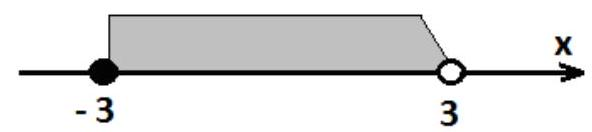
\includegraphics[max width=\textwidth, center]{2024_11_21_d45b0573b36a3462565cg-02}\\
c\\
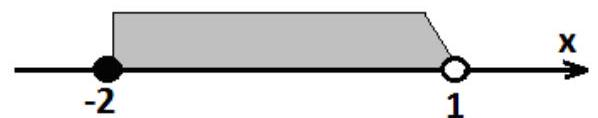
\includegraphics[max width=\textwidth, center]{2024_11_21_d45b0573b36a3462565cg-02(2)}\\
D\\
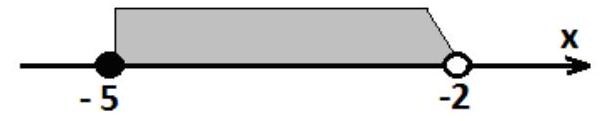
\includegraphics[max width=\textwidth, center]{2024_11_21_d45b0573b36a3462565cg-02(1)}

\section*{Zadanie 2. (1p)}
Wartość wyrażenia \(\log _{2} 16 \sqrt{2}-\log _{2} 2 \sqrt{2}\) jest równa\\
A. \(3^{-1}\)\\
B. \(\sqrt{3}\)\\
C. -3\\
D. 3

Zadanie 3. (1p)\\
Karolina ma o \(25 \%\) wyższy wynik z egzaminu próbnego od Oli. Wynika z tego, że Oli wynik jest niższy od wyniku Karoliny o\\
A. \(20 \%\)\\
B. \(22 \frac{1}{2} \%\)\\
C. \(25 \%\)\\
D. \(17 \frac{1}{2} \%\)

Zadanie 4. (1p)\\
Jeżeli \(a-b=4\) i \(a^{2}-b^{2}=56\), to \(a+b\) jest równe\\
A. 12\\
B. 13\\
C. 14\\
D. 15

\section*{Zadanie 5. (1p)}
Rozwiązaniem układu równań \(\left\{\begin{array}{l}x-y=2 \\ y+2 x=4\end{array}\right.\) w prostokątnym układzie współrzędnych na płaszczyźnie jest\\
A. jeden punkt\\
B. dwa punkty\\
C. zbiór pusty\\
D. prosta \(y=x\)

\section*{Zadanie 6. (1p)}
Iloczyn wszystkich pierwiastków równania \(-2(x-1)(2 x+6)(5-x)=0\) jest równy\\
A. 15\\
B. 30\\
C. -30\\
D. -15

\section*{Zadanie 7. (1p)}
Rozwiązaniem równania \(4=\frac{2 a-4}{a+3}\) jest liczba\\
A. \(a=2\)\\
B. \(a=-3\)\\
C. \(a=-8\)\\
D. \(a=1\)

BRUDNOPIS (nie podlega ocenie)

\section*{Zadanie 8. (1p)}
Dziedziną funkcji, której wykres przedstawiono na rysunku jest\\
A. \(\langle-3,-1) \cup\langle 0,2)\)\\
B. \(\langle-3,2)\)\\
C. \(\langle-2,2\rangle\)\\
D. \(\langle-2,1\rangle\)\\
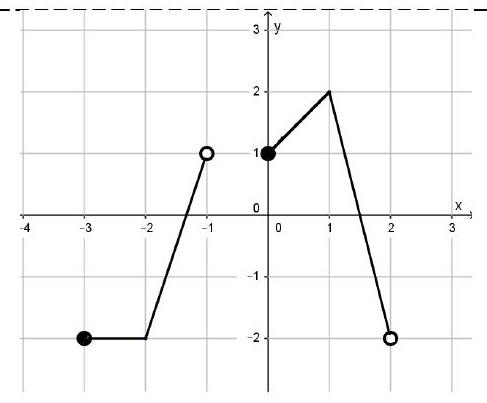
\includegraphics[max width=\textwidth, center]{2024_11_21_d45b0573b36a3462565cg-04(1)}

\section*{Zadanie 9. (1p)}
Punkt o wspórtrędnych \((-2,4)\) należy do prostej \(y=x+2 a-1\) zatem\\
A. \(a=3 \frac{1}{2}\)\\
B. \(a=-3 \frac{1}{2}\)\\
C. \(a=\frac{1}{2}\)\\
D. \(a=-4\)

\section*{Zadanie 10. (1p)}
Liczba 4 jest miejscem zerowym funkcji liniowej \(f(x)=(5-m) x+8\). Wynika stąd, że\\
A. \(m=-8\)\\
B. \(m=-5\)\\
C. \(m=7\)\\
D. \(m=5\)

Zadanie 11. (1p)\\
Funkcja kwadratowa f przyjmuje wartość największą równą -5 dla argumentu równego 2. Wobec tego funkcja fopisana jest wzorem\\
A. \(f(x)=(x-2)^{2}-5\)\\
B. \(f(x)=-(x-2)^{2}+5\)\\
C. \(f(x)=-(x+2)^{2}-5\)\\
D. \(f(x)=-(x-2)^{2}-5\)

Zadanie 12. (1p)\\
Największą liczbą całkowitą spełniającą nierówność \(\frac{x+3}{2}<\frac{1-x}{3}\) jest\\
A. 1\\
B. -2\\
C. 2\\
D. -1

\section*{Zadanie 13. (1p)}
Dany jest ciąg liczbowy \(\left(a_{n}\right)\), w którym \(a_{1}=3 x-9, a_{2}=6, a_{3}=3\). Dla jakiej wartości liczbowej x dany ciąg jest ciągiem geometrycznym?\\
A. \(x=7\)\\
B. \(x=8\)\\
C. \(x=6\)\\
D. \(x=5\)

\section*{Zadanie 14. (1p)}
Tangens kąta \(\alpha\) zaznaczonego na rysunku jest równy.\\
A. \(-\frac{2}{5}\)\\
B. \(\frac{5}{2}\)\\
C. \(\frac{2}{5}\)\\
D. \(-\frac{5}{2}\)\\
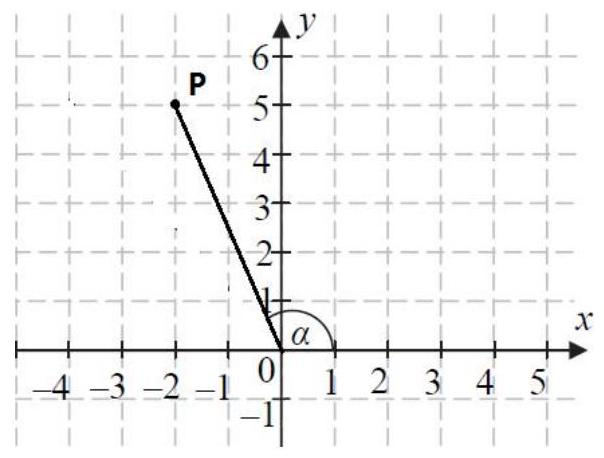
\includegraphics[max width=\textwidth, center]{2024_11_21_d45b0573b36a3462565cg-04}

BRUDNOPIS (nie podlega ocenie)

\section*{LUBELSKA PRÓBA PRZED MATURĄ 2017 - poziom podstawowy}
\section*{Zadanie 15. (1p)}
Jeżeli \(\operatorname{tg} \alpha=3 \sin \alpha\), oraz \(\alpha\) jest kątem ostrym, to\\
A. \(\cos \alpha=\frac{1}{2}\)\\
B. \(\cos \alpha=\frac{2}{3}\)\\
C. \(\cos \alpha=\frac{1}{3}\)\\
D. \(\cos \alpha=\frac{\sqrt{2}}{2}\)

Zadanie 16. (1p)\\
Jeżeli suma miar kąta środkowego i kąta wpisanego opartych na tym samym łuku jest równa \(180^{\circ}\), to kąty te są oparte na\\
A. \(\frac{1}{2}\) okręgu\\
B. \(\frac{1}{3}\) okregu\\
C. \(\frac{2}{3}\) okregu\\
D. \(\frac{1}{4}\) okreqgu

\section*{Zadanie 17. (1p)}
Przekątna prostokąta ma długość 12 cm i tworzy z jednym z boków kąt o mierze \(30^{\circ}\). Pole powierzchni tego prostokąta jest równe\\
A. \(36 \sqrt{3} \mathrm{~cm}^{2}\)\\
B. \(24 \sqrt{3} \mathrm{~cm}^{2}\)\\
C. \(36 \sqrt{2} \mathrm{~cm}^{2}\)\\
D. \(24 \sqrt{2} \mathrm{~cm}^{2}\)

Zadanie 18. (1p)\\
Proste o równaniach: \(y=a^{2} x-5\) i \(y=\frac{1}{2 a} x+4(a \neq 0)\) są prostopadłe dla \(\boldsymbol{a}\) równego\\
A. -1\\
B. 2\\
C. 1\\
D. -2

Zadanie 19. (1p)\\
Suma dwóch początkowych wyrazów ciągu arytmetycznego \(\left(a_{n}\right)\) wynosi 5 , a trzeci wyraz jest równy 7. Wówczas\\
A. \(a_{5}=13\)\\
B. \(a_{5}=12\)\\
C. \(a_{5}=11\)\\
D. \(a_{5}=14\)

Zadanie 20. (1p)\\
Środkiem odcinka o końcach \(A=(-4,8)\) i \(B=(a+3,4-2 b)\) jest początek prostokątnego układu współrzędnych. Wówczas\\
A. \(a=1, b=5\)\\
B. \(a=1, b=6\)\\
C. \(a=2, b=5\)\\
D. \(a=6, b=1\)

\section*{Zadanie 21. (1p)}
Dany jest graniastosłup prawidłowy czworokątny. (patrz rysunek) Podaj oznaczenie kąta zawartego między przekątną graniastosłupa i krawędzią podstawy.\\
A. kąt CAG\\
B. kąt HFG\\
C. kąt AGB\\
D. kąt GAB\\
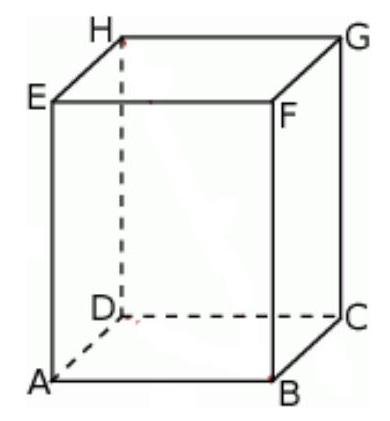
\includegraphics[max width=\textwidth, center]{2024_11_21_d45b0573b36a3462565cg-06}

BRUDNOPIS (nie podlega ocenie)

\section*{LUBELSKA PRÓBA PRZED MATURĄ 2017 - poziom podstawowy}
\section*{Zadanie 22. (1p)}
Pole przekroju osiowego walca jest równe 12. Pole powierzchni bocznej tego walca jest równe\\
A. \(10 \pi\)\\
B. \(16 \pi\)\\
C. \(12 \pi\)\\
D. \(24 \pi\)

\section*{Zadanie 23. (1p)}
Przekątna graniastosłupa prawidłowego czworokątnego o długości równej 10 cm jest nachylona do płaszczyzny podstawy pod kątem \(\alpha=60^{\circ}\). Wysokość tego graniastosłupa ma długość równą\\
A. \(5 \sqrt{3} \mathrm{~cm}\)\\
B. 5 cm\\
C. \(\frac{5 \sqrt{3}}{3} \mathrm{~cm}\)\\
D. \(5 \sqrt{2} \mathrm{~cm}\)

\section*{Zadanie 24. (1p)}
Dla jakiej wartości liczbowej x średnia arytmetyczna liczb: \(2,2,3,4,5,5,5, x\) jest równa 4 ?\\
A. 3\\
B. 4\\
C. 5\\
D. 6

Zadanie 25. (1p)\\
Losujemy rzucając dwukrotnie symetryczną kostką sześcienną. Jakie jest prawdopodobieństwo, że w drugim rzucie wylosujemy o trzy oczka więcej niż w pierwszym?\\
A. \(\frac{1}{36}\)\\
B. \(\frac{1}{18}\)\\
C. \(\frac{1}{12}\)\\
D. \(\frac{1}{4}\)

\section*{BRUDNOPIS (nie podlega ocenie)}
\section*{LUBELSKA PRÓBA PRZED MATURĄ 2017 - poziom podstawowy}
\section*{ZADANIA OTWARTE}
Rozwiqzania zadań o numerach od 26 do 34 należy zapisać \(w\) wyznaczonych miejscach pod treścia zadania (pamiętaj o udzieleniu odpowiedzi)

\section*{Zadanie 26. (2p)}
Rozwiąż nierówność \((x-2)^{2} \geq(x-2)(2 x+1)\).

Odpowiedź:

\section*{Zadanie 27. (2p)}
Wykaż, że dla dowolnych liczb całkowitych a, b liczba \(x=(2 a-b)^{2}-(a-2 b)^{2}\) jest podzielna przez 3.\\

\includegraphics[max width=\textwidth, center]{2024_11_21_d45b0573b36a3462565cg-09}

Zadanie 28. (2p)\\
Wykaż, że stosunek długości promienia okręgu wpisanego w kwadrat do długości promienia okręgu opisanego na tym kwadracie jest równy \(\frac{\sqrt{2}}{2}\).

\section*{LUBELSKA PRÓBA PRZED MATURĄ 2017 - poziom podstawowy}
\section*{Zadanie 29. (2p)}
Oblicz najmniejszą i największą wartość funkcji kwadratowej \(f(x)=x^{2}-2 x-3\) w przedziale \(\langle-3,1\rangle\).

Odpowiedź:

\section*{Zadanie 30. (2p)}
Dane są punkty \(A=(10,20)\) i \(B=(15,45)\). Wyznacz współrzędne punktu przecięcia prostej \(A B\) z osią \(O x\).

\section*{Zadanie 31. (2p)}
Średnia arytmetyczna dwóch liczb wynosi 16. Jeśli jedną z nich zmniejszymy dwukrotnie, a drugą zwiększymy o \(50 \%\), to średnia arytmetyczna zwiększy się o 2 . Wyznacz te liczby.\\

\includegraphics[max width=\textwidth, center]{2024_11_21_d45b0573b36a3462565cg-10}

Odpowiedź:

\section*{LUBELSKA PRÓBA PRZED MATURĄ 2017 - poziom podstawowy}
\section*{Zadanie 32. (4p)}
W graniastosłupie prawidłowym trójkątnym przekątna ściany bocznej tworzy z płaszczyzną podstawy kąt o mierze równej \(45^{\circ}\). Oblicz pole powierzchni bocznej tego graniastosłupa, wiedząc, że jego objętość jest równa \(16 \sqrt{3}\).

Odpowiedź:

\section*{LUBELSKA PRÓBA PRZED MATURĄ 2017 - poziom podstawowy}
\section*{Zadanie 33. (4p)}
Ze zbioru \(D=\{-3,-2,-1,1,2\}\) losujemy najpierw jedną liczbę i oznaczamy ją jako \(\boldsymbol{a}\). Następnie z pozostałych liczb losujemy drugą liczbę i oznaczamy ją jako \(\boldsymbol{b}\). Liczby \(\boldsymbol{a}\) i \(\boldsymbol{b}\) są współczynnikami funkcji kwadratowej \(f(x)=a x^{2}+b\). Oblicz prawdopodobieństwo zdarzenia:\\
a) X - funkcja \(f\) jest malejąca w zbiorze \(\langle 0,+\infty)\).\\
b) Y - funkcja \(f\) ma dwa różne miejsca zerowe.

\section*{LUBELSKA PRÓBA PRZED MATURĄ 2017 - poziom podstawowy}
\section*{Zadanie 34. (5p)}
Cąag \(\left(a_{n}\right)\), gdzie \(n \in N_{+}\), jest nieskończonym ciągiem arytmetycznym o różnicy 2, w którym pierwszy wyraz jest równy -10 . Wyznacz wszystkie wartości \(\boldsymbol{k}\), dla których trzywyrazowy ciąg \(\left(a_{k+1}, a_{k+3}, a_{2 k+3}\right)\) jest ciaggiem geometrycznym.

Odpowiedź:

\section*{BRUDNOPIS (nie podlega ocenie)}
\section*{BRUDNOPIS (nie podlega ocenie)}
KARTA ODPOWIEDZI

KOD UCZNIA \(\square\) Nazwisko iimię

Wypelnia piszący

\begin{center}
\begin{tabular}{|c|c|c|c|c|}
\hline
\begin{tabular}{c}
Nr \\
zadmia \\
\end{tabular} & A & B & C & D \\
\hline
1. & \(\square\) & \(\square\) & \(\square\) & \(\square\) \\
\hline
2. & \(\square\) & \(\square\) & \(\square\) & \(\square\) \\
\hline
3. & \(\square\) & \(\square\) & \(\square\) & \(\square\) \\
\hline
4. & \(\square\) & \(\square\) & \(\square\) & \(\square\) \\
\hline
5. & \(\square\) & \(\square\) & \(\square\) & \(\square\) \\
\hline
6. & \(\square\) & \(\square\) & \(\square\) & \(\square\) \\
\hline
7. & \(\square\) & \(\square\) & \(\square\) & \(\square\) \\
\hline
8. & \(\square\) & \(\square\) & \(\square\) & \(\square\) \\
\hline
9. & \(\square\) & \(\square\) & \(\square\) & \(\square\) \\
\hline
10. & \(\square\) & \(\square\) & \(\square\) & \(\square\) \\
\hline
11. & \(\square\) & \(\square\) & \(\square\) & \(\square\) \\
\hline
12. & \(\square\) & \(\square\) & \(\square\) & \(\square\) \\
\hline
13. & \(\square\) & \(\square\) & \(\square\) & \(\square\) \\
\hline
14. & \(\square\) & \(\square\) & \(\square\) & \(\square\) \\
\hline
15. & \(\square\) & \(\square\) & \(\square\) & \(\square\) \\
\hline
16. & \(\square\) & \(\square\) & \(\square\) & \(\square\) \\
\hline
17. & \(\square\) & \(\square\) & \(\square\) & \(\square\) \\
\hline
18. & \(\square\) & \(\square\) & \(\square\) & \(\square\) \\
\hline
19. & \(\square\) & \(\square\) & \(\square\) & \(\square\) \\
\hline
20. & \(\square\) & \(\square\) & \(\square\) & \(\square\) \\
\hline
21. & \(\square\) & \(\square\) & \(\square\) & \(\square\) \\
\hline
22. & \(\square\) & \(\square\) & \(\square\) & \(\square\) \\
\hline
23. & \(\square\) & \(\square\) & \(\square\) & \(\square\) \\
\hline
24. & \(\square\) & \(\square\) & \(\square\) & \(\square\) \\
\hline
25. & \(\square\) & \(\square\) & \(\square\) & \(\square\) \\
\hline
\end{tabular}
\end{center}

Razem \(\square\)

Wypelnia sprawdzający

\begin{center}
\begin{tabular}{|c|c|c|c|c|}
\hline
\begin{tabular}{c}
\(\mathrm{Nr}_{\mathrm{r}}\) \\
\end{tabular} & X & 0 & 1 & 2 \\
\hline
zadmis & X & \(\square\) & \(\square\) & \(\square\) \\
\hline
26. & \(\square\) & \(\square\) & \(\square\) & \(\square\) \\
\hline
27. & \(\square\) & \(\square\) & \(\square\) & \(\square\) \\
\hline
28. & \(\square\) & \(\square\) & \(\square\) & \(\square\) \\
\hline
29. & \(\square\) & \(\square\) & \(\square\) & \(\square\) \\
\hline
30. & \(\square\) & \(\square\) & \(\square\) & \(\square\) \\
\hline
31. & \(\square\) & \(\square\) & \(\square\) & \(\square\) \\
\hline
\end{tabular}
\end{center}

Razem\\
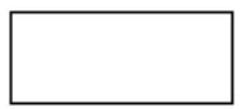
\includegraphics[max width=\textwidth, center]{2024_11_21_d45b0573b36a3462565cg-16}

\begin{center}
\begin{tabular}{|c|c|c|c|c|c|c|c|}
\hline
\begin{tabular}{c}
Nr \\
Zadamia \\
\end{tabular} & X & 0 & 1 & 2 & 3 & 4 & 5 \\
\hline
32. & \(\square\) & \(\square\) & \(\square\) & \(\square\) & \(\square\) & \(\square\) &  \\
\hline
33. & \(\square\) & \(\square\) & \(\square\) & \(\square\) & \(\square\) & \(\square\) &  \\
\hline
34. & \(\square\) & \(\square\) & \(\square\) & \(\square\) & \(\square\) & \(\square\) & \(\square\) \\
\hline
\end{tabular}
\end{center}

Razem \(\square\)


\end{document}